% !TEX root = ../main.tex
% !TEX root = ../main.tex
\begin{figure}[t]
\vspace{-0.5in}
\centering
\iflatexml
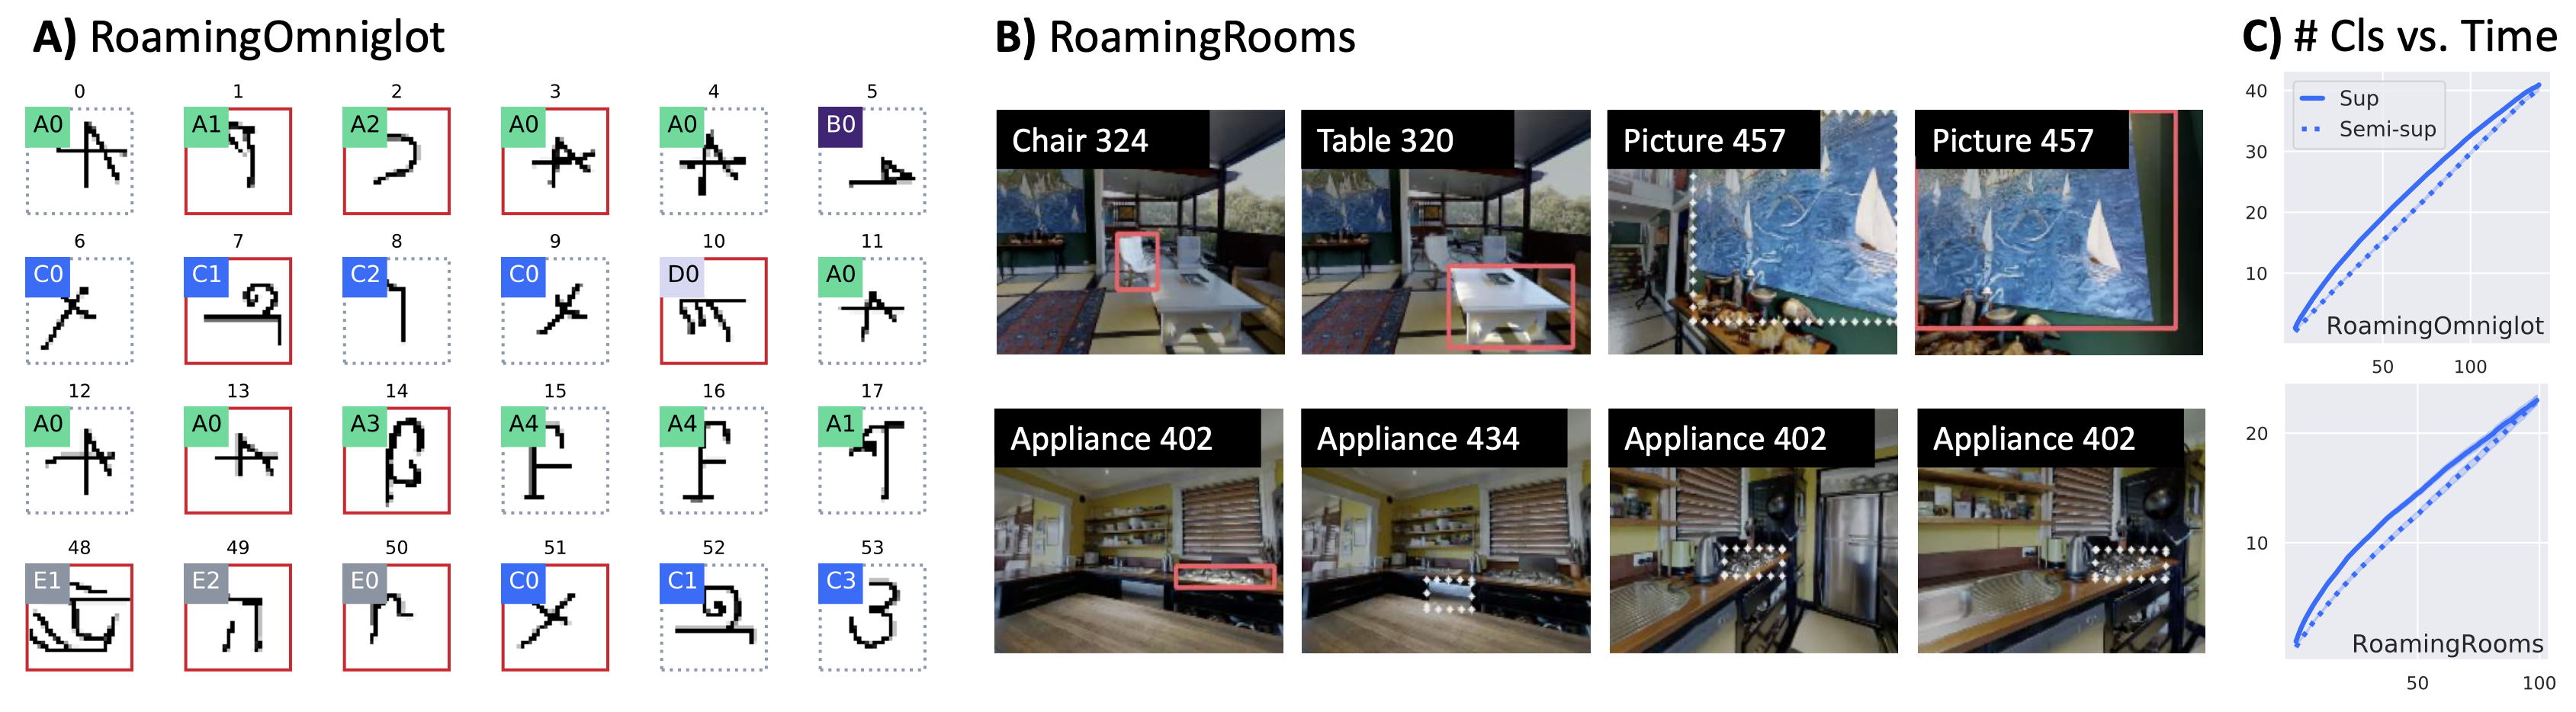
\includegraphics[width=6\textwidth]{figures/datasets-copy-samll-compressed-2.png}
\else
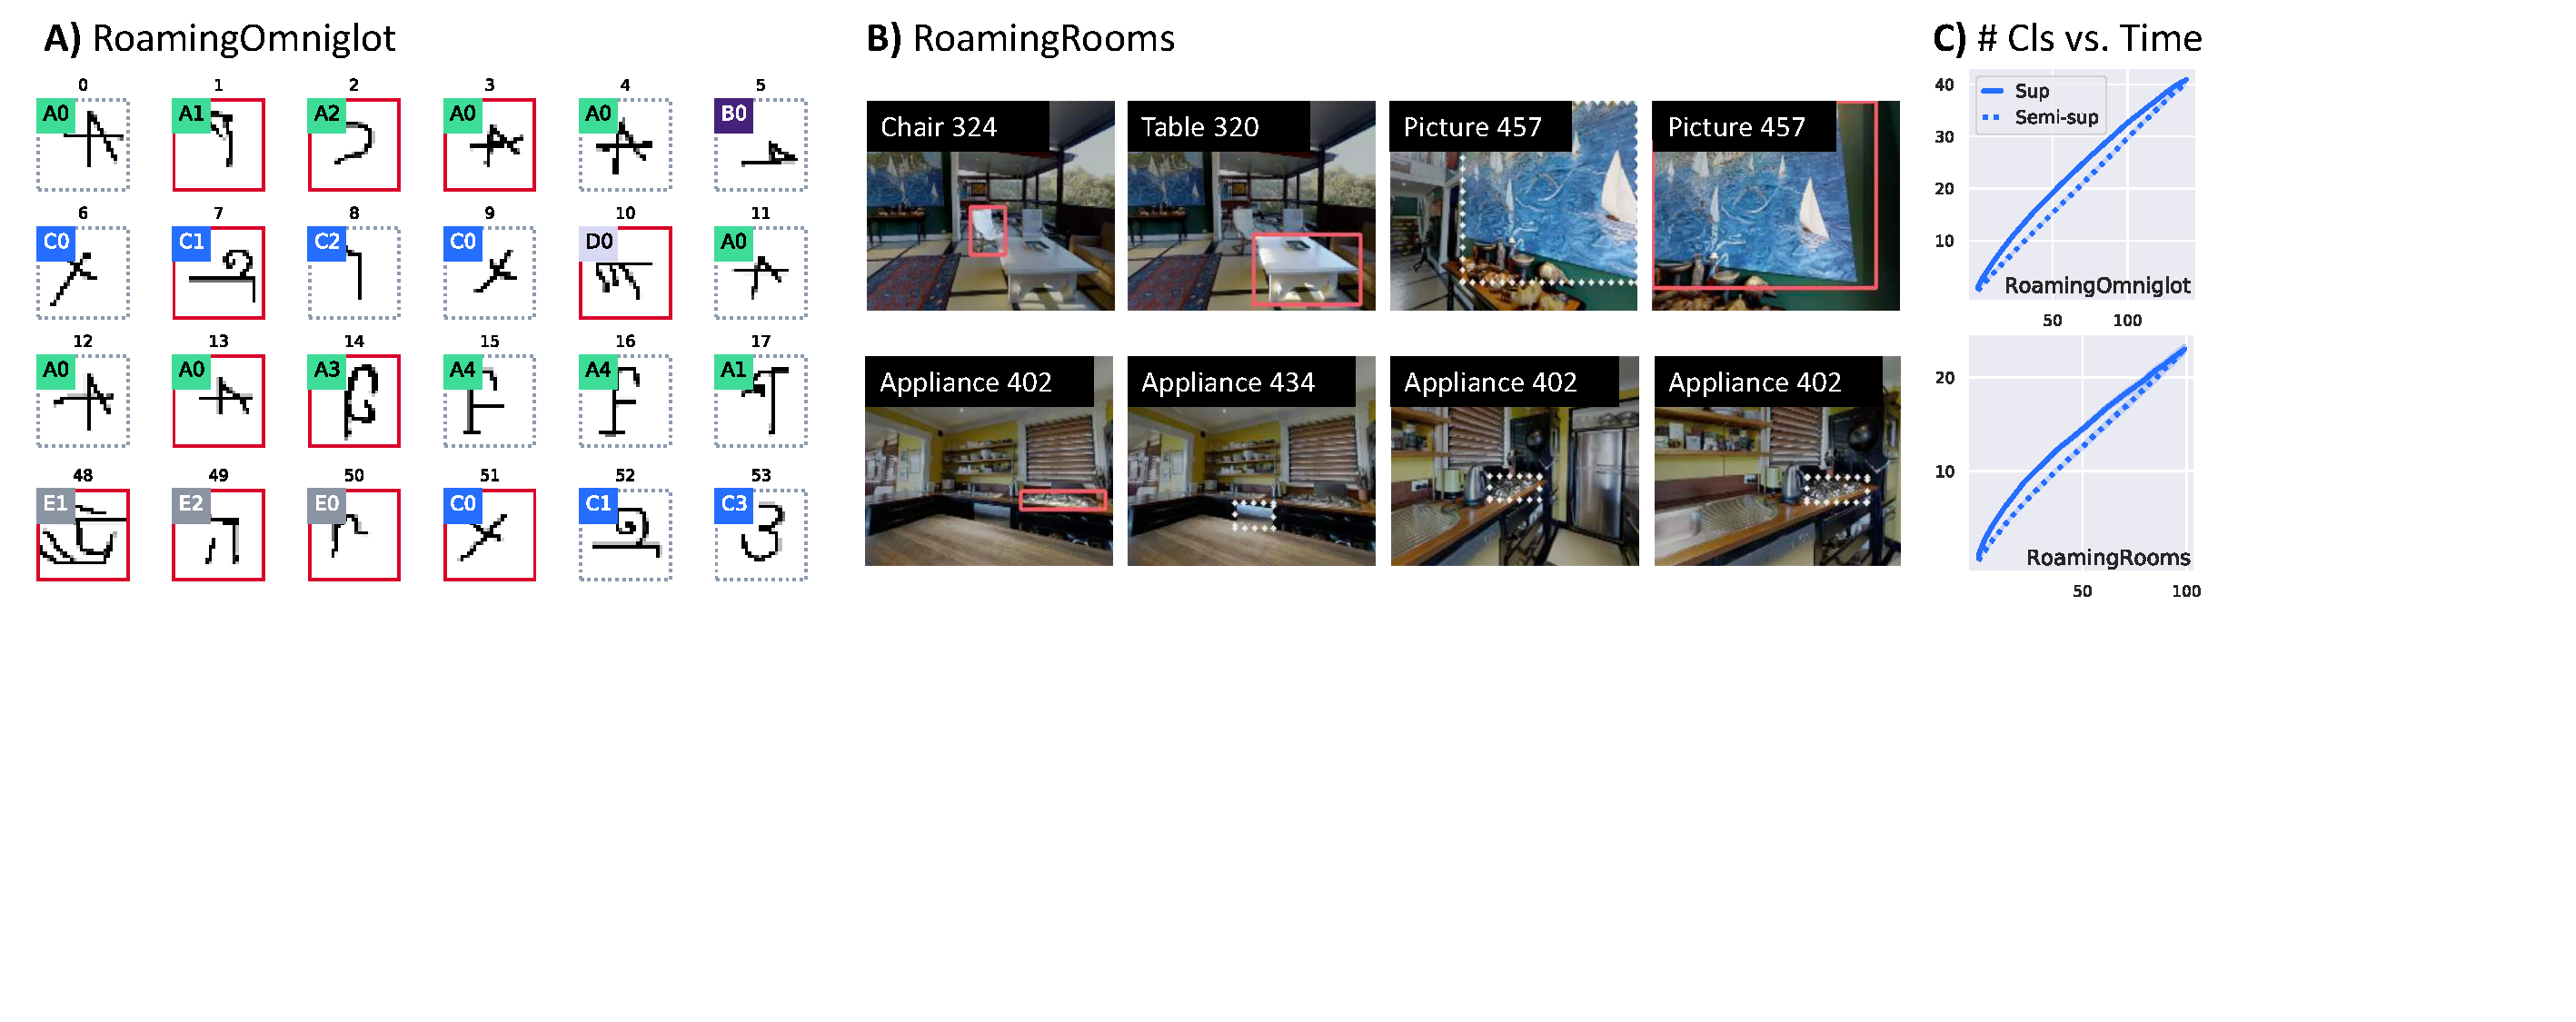
\includegraphics[width=\textwidth, trim={0cm 7cm 6.5cm 0}, clip]{figures/datasets-copy-small-compressed-2.pdf}
\fi
\vspace{-0.32in}
\caption{\looseness=-1 \textbf{Sample online contextualized few-shot learning sequences.} \textbf{A)}
\ourchar{}. Red solid boxes denote labeled examples of Omniglot handwritten characters, and
dotted boxes denote unlabeled ones. Environments are shown in colored labels in the top left corner.
\textbf{B)} Image frame samples of a few-shot learning sequence in our \ourroom{} dataset collected
from a random walking agent. The task here is to recognize and classify novel instance IDs in the home environment. Here the groundtruth instance masks/bounding boxes are provided.
\textbf{C)} The growth of total number of labeled classes in a sequence for \ourchar{} (top) and
\ourroom{} (bottom).}
\label{fig:dataset}
\vspace{-0.15in}
\end{figure}

\section{Related Work}
\vspace{-0.1in}
In this section, we briefly review paradigms that have been used for few-shot learning (FSL) and
continual learning (CL). 
% Table~\ref{tab:benchmark} compares these paradigms based on various
% properties of the task; To denote properties that are incorporated in some preliminary form, we use
% {\smash\tinyhm{}} to denote properties that are not fully implemented but have some preliminary
% form. For example, the class-incremental learning paradigm evaluates models after each task  is
% completed, which is similar to our online evaluation in spirit but still not the same  as the
% evaluation does not take place after each example. 
% Our proposed \emph{online contextual few-shot
% learning (OC-FSL)} spans the complete set of features of the other paradigms. We also review
% relevant models and their relationship to our \ourmodelshort.
% % !TEX root = ../main.tex
\begin{table*}[t]
\iflatexml
    \begin{tabular}{ccccccc}
    \toprule
    \mr{2}{\tb{Tasks}}                     & \tb{Few}  & \tb{Semi-sup. } & \mr{2}{\tb{Continual}} & \tb{Online} & \tb{Predict}& \tb{Soft Context}  \\
                                           & \tb{Shot} & \tb{Supp. Set}  &                        & \tb{Eval.}  & \tb{New}    & \tb{Switch}        \\
    \midrule                                                                                                                                                                          
    Incremental Learning (IL) \citep{icarl}& \xm       & \xm             & \cm                    & \hx         & \xm         & \xm                \\
    Few-shot (FSL) \citep{matchingnet}     & \cm       & \xm             & \xm                    & \xm         & \xm         & \xm                \\
    Incremental FSL \citep{attnattractor}  & \cm       & \xm             & \hx                    & \xm         & \xm         & \xm                \\
    Cls. Incremental FSL \citep{fscil}     & \cm       & \xm             & \cm                    & \hx         & \xm         & \xm                \\
    Semi-supv. FSL \citep{fewshotssl}      & \cm       & \cm             & \xm                    & \xm         & \cm         & \xm                \\
    MOCA \citep{moca}                      & \cm       & \xm             & \cm                    & \xm         & \xm         & \hx                \\
    Online Mixture \citep{onlinemixture}   & \cm       & \xm             & \cm                    & \xm         & \xm         & \hx                \\
    Online Meta \citep{oml}                & \cm       & \xm             & \cm                    & \xm         & \xm         & \xm                \\
    Continual FSL* \citep{contfsl}         & \cm       & \xm             & \cm                    & \xm         & \xm         & \xm                \\
    OSAKA* \citep{osaka}                   & \cm       & \xm             & \cm                    & \cm         & \hx         & \cm                \\
    \midrule                                                                                                                                                                                         
    OC-FSL (Ours)                          & \cm       & \cm             & \cm                    & \cm         & \cm         & \cm                \\
    \bottomrule
    \end{tabular}
    \caption{Comparison of past FSL and CL paradigms vs. our online contextualized FSL (OC-FSL). * denotes concurrent work.}
    \label{tab:benchmark}
\else
    \vspace{-0.5in}
    \caption{Comparison of past FSL and CL paradigms vs. our online contextualized FSL (OC-FSL).}
    \begin{center}
    \begin{small}
    \resizebox{\textwidth}{!}{
    \begin{tabular}{ccccccc}
    \toprule
    \mr{2}{\tb{Tasks}}                     & \tb{Few}  & \tb{Semi-sup. } & \mr{2}{\tb{Continual}} & \tb{Online} & \tb{Predict}& \tb{Soft Context}  \\
                                           & \tb{Shot} & \tb{Supp. Set}  &                        & \tb{Eval.}  & \tb{New}    & \tb{Switch}        \\
    \midrule                                                                                                                                                                          
    Incremental Learning (IL) \citep{icarl}& \xm       & \xm             & \cm                    & \hx         & \xm         & \xm                \\
    Few-shot (FSL) \citep{matchingnet}     & \cm       & \xm             & \xm                    & \xm         & \xm         & \xm                \\
    Incremental FSL \citep{attnattractor}  & \cm       & \xm             & \hx                    & \xm         & \xm         & \xm                \\
    Cls. Incremental FSL \citep{fscil}     & \cm       & \xm             & \cm                    & \hx         & \xm         & \xm                \\
    Semi-supv. FSL \citep{fewshotssl}      & \cm       & \cm             & \xm                    & \xm         & \cm         & \xm                \\
    MOCA \citep{moca}                      & \cm       & \xm             & \cm                    & \xm         & \xm         & \hx                \\
    Online Mixture \citep{onlinemixture}   & \cm       & \xm             & \cm                    & \xm         & \xm         & \hx                \\
    Online Meta \citep{oml}                & \cm       & \xm             & \cm                    & \xm         & \xm         & \xm                \\
    Continual FSL* \citep{contfsl}         & \cm       & \xm             & \cm                    & \xm         & \xm         & \xm                \\
    OSAKA* \citep{osaka}                   & \cm       & \xm             & \cm                    & \cm         & \hx         & \cm                \\
    \midrule                                                                                                                                                                                         
    OC-FSL (Ours)                          & \cm       & \cm             & \cm                    & \cm         & \cm         & \cm                \\
    \bottomrule
    \end{tabular}
    }
    \label{tab:benchmark}
    \\
    \vspace{0.05in}
    * denotes concurrent work.
    \end{small}
    \end{center}
\fi
\end{table*}


\vspace{-0.1in}
\paragraph{Few-shot learning:} 
FSL~\citep{omniglot,generativefewshot,siamese,matchingnet} considers learning new tasks with few
labeled examples. FSL models can be categorized as based on: metric
learning~\citep{matchingnet,protonet}, memory~\citep{mann}, and gradient
adaptation~\citep{maml,metasgd}. The model we propose, \ourmodelshort, lies on the boundary between
these approaches, as we use an RNN to model the temporal context but we also use metric-learning
mechanisms and objectives to train.

Several previous efforts have aimed to extend few-shot learning to incorporate more natural
constraints. One such example is semi-supervised FSL~\citep{fewshotssl}, where models also learn 
% not only
% from a few labeled examples but also 
from a pool of unlabeled examples. While traditional FSL only
tests the learner on novel classes, \emph{incremental FSL}~\citep{lwof,attnattractor} tests on novel
classes together with a set of base classes. These approaches, however, have not explored how to
iteratively add new classes.

In concurrent work, \citet{contfsl} extend FSL to a continual setting based on image sequences, each
of which is divided into stages with a fixed number of examples per class followed by a query set. It
focuses on more flexible and faster adaptation since the models are evaluated online, and the context is
a soft constraint instead of a hard separation of tasks. Moreover, new classes need to be identified
as part of the sequence, crucial to any learner's incremental acquisition of knowledge.

\vspace{-0.1in}
\paragraph{Continual learning:} Continual (or lifelong) learning is a parallel line of research that
aims to handle a sequence of dynamic tasks~\citep{ewc,lwf,gem,expandable}. A key challenge here is
catastrophic forgetting~\citep{mccloskey1989catastrophic}, where the model ``forgets'' a task that
has been learned in the past. Incremental learning~\citep{icarl,eeil,bic,rebalance,inconline} is a
form of continual learning, where each task is an incremental batch of several new classes. This
assumption that novel classes always come in batches seems unnatural.

Traditionally, continual learning is studied with tasks such as permuted MNIST~\citep{mnist} or
split-CIFAR~\citep{cifar}. Recent datasets aim to consider more realistic continual learning, such as
CORe50~\citep{core50} and OpenLORIS~\citep{openloris}. We summarize core features of these continual
learning datasets in Appendix~\ref{app:data}. First, both CORe50 and OpenLORIS have relatively few object
classes, which makes meta-learning approaches inapplicable; second, both contain images of
small objects with minimal occlusion and viewpoint changes; and third, OpenLORIS does not have the
desired incremental class learning.

In concurrent work, \citet{osaka} proposes a setup to unify continual learning and meta-learning with
a similar online evaluation procedure. However, there are several notable differences. First, their
models focus on a general loss function without a specific design for predicting new classes; they
predict new tasks by examining if the loss of %the current prediction 
exceeds some threshold.
Second, the sequences of inputs are fully supervised. %, which allows their models to evaluate the loss
%function every step. 
Lastly, their benchmarks are based on synthetic task sequences such as Omniglot or tiered-ImageNet, which are less naturalistic than our RoamingRooms dataset.

\vspace{-0.1in}
\paragraph{Online meta-learning:}
Some existing work builds on early approaches~\citep{thrun,Schmidhuber1987evolutionary} that tackle
continual learning from a meta-learning perspective. \citet{onlinemeta} proposes storing all task
data in a data buffer%to perform inner loop gradient descent
; by contrast, \citet{oml} proposes to
%directly update the inner loop with the current input and 
instead learn a good representation that
supports such online updates. In \citet{onlinemixture}, a hierarchical Bayesian mixture model is used
to address the dynamic nature of continual learning. 
% To evaluate the performance of online
% meta-learning methods, the papers above also created a few synthetic continual learning tasks, which
% are less realistic than ours (see Table~\ref{tab:benchmark}).

\vspace{-0.1in}
\paragraph{Connections to the human brain:}
Our \ourmodelshort\ model consists of multiple memory systems, consistent with claims of cognitive
neuroscientists of multiple memory systems in the brain. The  complementary learning systems (CLS)
theory~\citep{cls} suggests that the hippocampus stores the recent experience and is likely where
few-shot learning takes place. However, our model is more closely related to contextual binding
theory~\citep{ctxbinding}, which suggests that long-term encoding of information depends on binding
spatiotemporal context, and without this context as a cue, forgetting occurs. Our proposed
\ourmodelshort\ contains parallels to human brain memory components~\citep{cohensquire}. Long term
statistical learning is captured in a CNN that produces a deep embedding. An RNN holds a type of
working memory that can retain novel objects and spatiotemporal contexts. Lastly, the prototype
memory represents the semantic memory, which consolidates multiple events into a single knowledge
vector~\citep{semanticmem}. Other deep learning researchers have proposed multiple memory
systems for continual learning. In \citet{dualmem}, the learning algorithm is heuristic and
representations come from pretrained networks. In \citet{fearnet}, a prototype memory is used for
recalling recent examples and rehearsal from a generative model allows this knowledge to be
integrated and distilled into a long-term memory.